% !TEX root = ../main.tex
\section{Research Context: The Apify Store}
\label{sec:context}

This section describes the institutional setting, pricing architecture, and the
platform's access boundary that structure our analysis.

%% ─────────────────────────────────────────────
\subsection{Platform Overview}

Apify is a cloud automation platform providing serverless infrastructure for
web scrapers, browser automations, and data-extraction workflows. Developers
build discrete tools called \emph{actors}---self-contained programs that accept
structured input, execute a task, and return structured output---and publish
them to the \emph{Apify Store}, a public marketplace where end users discover,
configure, and run tools. The Store is a two-sided market: developers supply
actors and earn revenue from usage, while users pay on a usage or rental basis
(or use free actors) to access a growing catalog of pre-built automations.

%% ─────────────────────────────────────────────
\subsection{Pricing Architecture}

The Store supports three pricing models. \emph{Pay-per-event} (PPE) is the
dominant model (84\% of actors): developers define billable events and a
per-event price, so cost is proportional to output volume. The \emph{rental}
model (8\%) charges a flat monthly fee; Apify has announced its sunset for
October 2026, when remaining rental actors are migrated to pay-per-usage
pricing (developers may instead opt into PPE themselves). The remaining 8\% are
\emph{free}. Because agentic readiness is available only to PPE tools, our
analyses restrict to the PPE sample, which removes the pricing-model confound
by construction.

%% ─────────────────────────────────────────────
\subsection{Agentic Readiness: Which Tools Agents May Use}

The central platform design decision in our study is the boundary Apify draws
around its newest class of consumer: AI agents that autonomously discover,
invoke, and pay for tools. For a tool to be usable by an agent through the
platform's agentic-payment mode, it must first be \emph{agentic-ready}.
Apify's documented eligibility criteria\footnote{Apify, ``Agentic Payments,''
Apify Documentation, \url{https://docs.apify.com/integrations/skyfire}.} are
several and span three levels. At the \emph{tool} level, a tool must use
pay-per-event pricing, charge only for events rather than platform usage, run
with \emph{limited permissions}, and not use \emph{standby mode}. At the
\emph{developer} level, the publisher must complete identity verification
(KYC). At the \emph{approval} level, Apify maintains a curated list of tools
approved for agentic payments.

Among these, the two \emph{architectural} requirements---limited permissions
and no standby---are the criteria we study, because they are the ones a
developer sets directly in the tool's architecture and the ones that determine
whether a tool is \emph{built} to be safely and predictably invoked without
human oversight. Limited permissions restrict what the tool may access;
non-standby keeps its execution model synchronous and predictable. We define a
tool as \emph{agentic-ready} when it satisfies both architectural requirements
(and non-agentic-ready otherwise); we deliberately do not condition on KYC or
curation, which are platform-side gates operating at the developer and
approval levels rather than properties of the tool itself.

This operationalization captures \emph{architectural} admission---the tool-level
design boundary that separates tools built for machine consumption from those
that are not---rather than the platform's full approval decision. It is a
necessary-but-not-sufficient condition for agentic-payment eligibility: a tool
that fails either architectural criterion cannot be agentic-eligible, while a
tool that passes both may still be excluded by KYC or curation. The
architectural boundary is our object of study because it is the aspect of the
admission decision most visible to and controllable by the developer, and the
aspect through which the platform encodes a legible ``machine-readable''
interface for agents. We do not observe whether any agent actually invokes a
given tool---agentic readiness describes admission to the agent-accessible
set, not realized agent use.

As of our data collection, 50{,}917 of the 53{,}502 PPE tools with architecture
data (95\%) satisfy the two architectural criteria. In the platform's
agentic-payment mode, the Store API's \texttt{allowsAgenticUsers}
filter\footnote{Apify, ``Agentic Payments,'' Apify Documentation,
\url{https://docs.apify.com/integrations/skyfire}.} and the MCP
\texttt{search-actors} tool\footnote{Apify, ``Apify MCP Server,'' Apify
Documentation, \url{https://docs.apify.com/integrations/mcp}.} surface
agentic-eligible tools to dynamic agent discovery, and attempts to invoke
ineligible tools are rejected by the platform.

%% ─────────────────────────────────────────────
\subsection{Scale, Structure, and Developer Ecology}

\autoref{tab:overview} summarizes key marketplace metrics. The Store contains
67{,}609 actors built by 5{,}789 developers. Adoption is heavily right-skewed:
the median actor has one monthly user, while the mean is far higher, reflecting
extreme upper-tail concentration consistent with prior analyses of mobile-app
demand \cite{ghose2014apppricing} and the GPT Store \cite{su2024gptstore}.

\begin{table}[t]
  \centering
  \caption{Apify Store overview. Counts reflect the full census as of the data
    collection date. Agentic-readiness (limited-permission, non-standby) is
    measured among the 53{,}502 pay-per-event tools with architecture data.}
  \label{tab:overview}
  \small
  \begin{tabular}{l r}
    \toprule
    \textbf{Metric} & \textbf{Value} \\
    \midrule
    Total actors              & 67,609 \\
    Unique developers         & 5,789 \\
    Agentic-ready PPE actors (\%)  & 50,917 (95\%) \\
    Non-agentic-ready actors (\%) & 2,585 (5\%) \\
    PPE-priced actors (\%)     & 57,032 (84\%) \\
    Rental-priced actors (\%)  & 5,364 (8\%) \\
    Free actors (\%)           & 5,213 (8\%) \\
    Median monthly users per actor & 1 \\
    Categories                 & 25 \\
    \bottomrule
  \end{tabular}
\end{table}

Developer participation is similarly concentrated (\autoref{tab:dev_tiers}):
125 whale developers (100+ actors each) account for over half the marketplace,
while 2{,}732 solo developers have published a single actor each. This
whale--long-tail structure shapes the competitive environment: a small cohort
of prolific developers dominates aggregate adoption, while most developers run
single-tool micro-businesses.

\begin{table}[t]
  \centering
  \caption{Developer portfolio tiers. Portfolio size = number of actors
    published by a developer. Agentic-ready share = average share of a
    developer's pay-per-event actors that are agentic-ready (limited-permission,
    non-standby).}
  \label{tab:dev_tiers}
  \small
  \begin{tabular}{l r r r r}
    \toprule
    \textbf{Tier} & \textbf{Portfolio size} & \textbf{Developers} & \textbf{Actors} & \textbf{Agentic-ready (\%)} \\
    \midrule
    Solo       & 1          & 2,732 & 2,732 & 78.8\% \\
    Boutique   & 2--9       & 2,145 & 8,265 & 88.5\% \\
    Mid        & 10--99     & 787 & 21,283 & 94.3\% \\
    Whale      & 100+       & 125 & 35,329 & 97.9\% \\
    \bottomrule
  \end{tabular}
\end{table}

\autoref{fig:usage_dist} shows the log-transformed distribution of monthly
users across the PPE analysis sample, illustrating the heavy right tail.
\autoref{fig:categories} shows category composition, with the agentic-ready
share within each major category.

\begin{figure}[t]
  \centering
  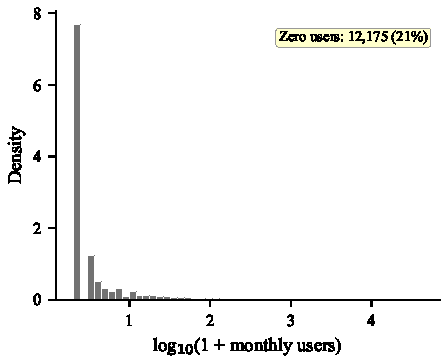
\includegraphics[width=0.7\columnwidth]{figures/F1_usage_distribution}
  \caption{Distribution of monthly users across the 57{,}032 PPE actors (log
    scale). The median actor has one monthly user; the distribution exhibits a
    heavy right tail spanning four orders of magnitude.}
  \label{fig:usage_dist}
\end{figure}

\begin{figure}[t]
  \centering
  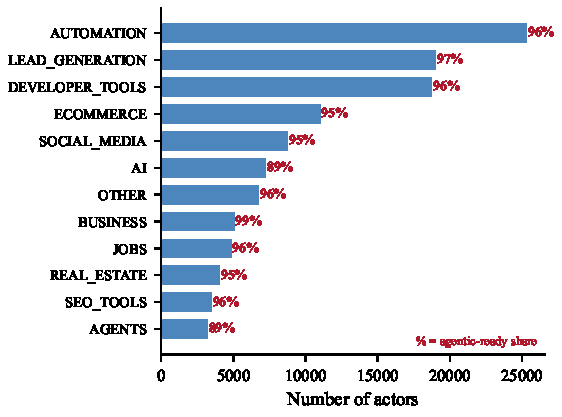
\includegraphics[width=0.7\columnwidth]{figures/F2_category_composition}
  \caption{Category composition of the Apify Store. Bar height shows total
    actor count per category; percentage labels show the agentic-ready share of
    each category.}
  \label{fig:categories}
\end{figure}

%% ─────────────────────────────────────────────
\subsection{Representativeness and Boundary Conditions}

Apify is one of several automation marketplaces (Zapier, UiPath Marketplace,
Bardeen) sharing the structural properties identified in
\autoref{sec:bg:automation}; it is distinctive in providing a public, crawlable
marketplace with tool-level metadata and an explicit agent-accessible boundary.
One boundary condition is that Apify is not an app store: actors are headless
scripts consumed through API calls, not interactive applications, so the
findings apply most directly to headless automation marketplaces.

%% ─────────────────────────────────────────────
\subsection{The Rental Sunset}

A concurrent institutional change provides context: Apify has announced the
deprecation of rental pricing (October 2026),\footnote{Apify, ``Rental Pricing
Model,'' Apify Documentation,
\url{https://docs.apify.com/actors/publishing/monetize/rental}.} at which point
the remaining 5{,}364 rental actors (8\% of the marketplace) are migrated to
pay-per-usage pricing. Developers who instead want the pay-per-event model must
actively migrate their actors themselves. A rental actor that a developer
converts to pay-per-event becomes eligible for agentic readiness only if it is
also configured with limited permissions and no standby; its full effects unfold
after our observation window.
